\begin{flushright} {\tiny {\color{gray} \tt mars\_structure.tex}} \end{flushright}
%~~~~~~~~~~~~~~~~~~~~~~~~~~~~~~~~~~~~~~~~~~~~~~~~~~~~~~~~~~~~~~~~~~~~~~~~~~~~~~~~~

\begin{itemize}

%------------------------------
\item \fullcite{domk18}

\begin{displayquote}
{\color{darkgray}
Mars' radius (\~{}3390 km) is about half that of the Earth, and it 
has nearly 1/8 of Earth's mass. Though a lack of seismic information 
means that its interior structure and composition are not well known 
as Earth's, Mars is, nevertheless, inferred to be a differentiated 
planetary body. It has a core estimated to be nearly the same radius 
as Earth's solid inner core (\~{}1200 km); a thinner mantle (\~{}2100 km), 
about \~{}2/3 that of Earth (\~{}2100 km); and a thicker crust, nearly 
double or more than that of Earth, reaching more than 60 km thick 
in parts of the southern cratered highlands. Oceanic-type crust has 
been interpreted to be roughly representative of the northern plains, 
while continental crust has been hypothesized to underlie the southern highlands 
}
\end{displayquote}

\begin{center}
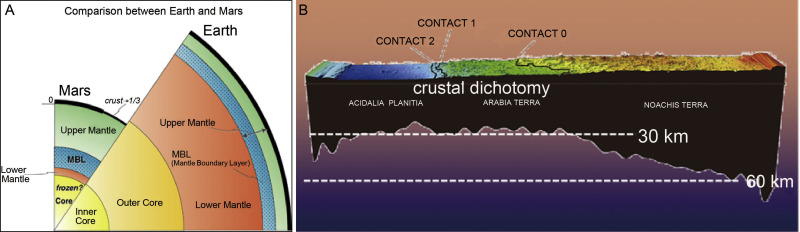
\includegraphics[width=14cm]{images/mars/domk18b}\\
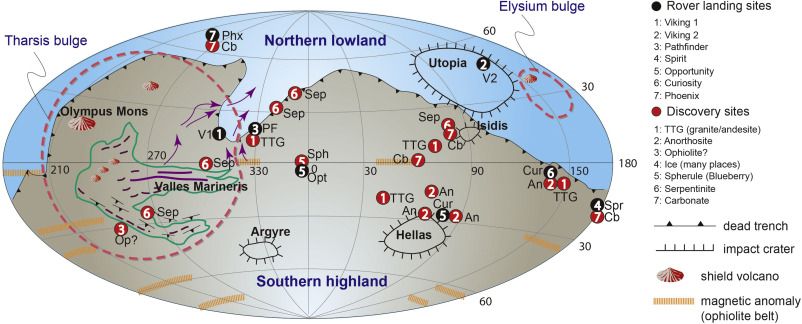
\includegraphics[width=12cm]{images/mars/domk18a}
\end{center}

%------------------------------
\item \fullcite{plpt18}

\begin{center}
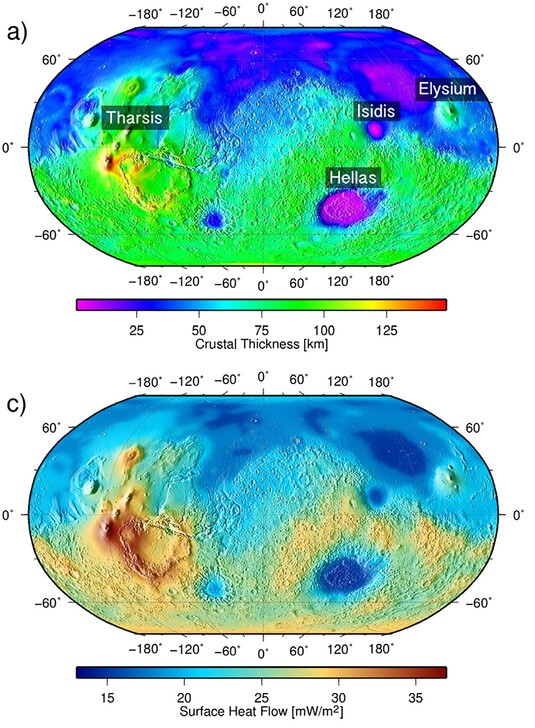
\includegraphics[width=6cm]{images/mars/plpt18}
\end{center}

%------------------------------
\item \fullcite{dilg19}

\begin{center}
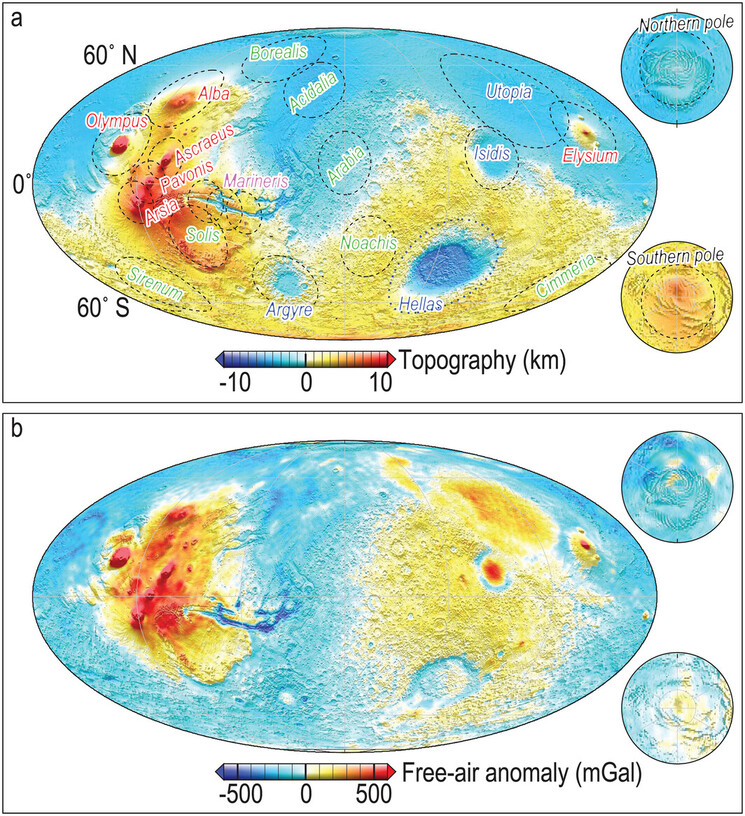
\includegraphics[width=6cm]{images/mars/dilg19}
\end{center}

%------------------------------
\item \fullcite{smls19}

\begin{center}
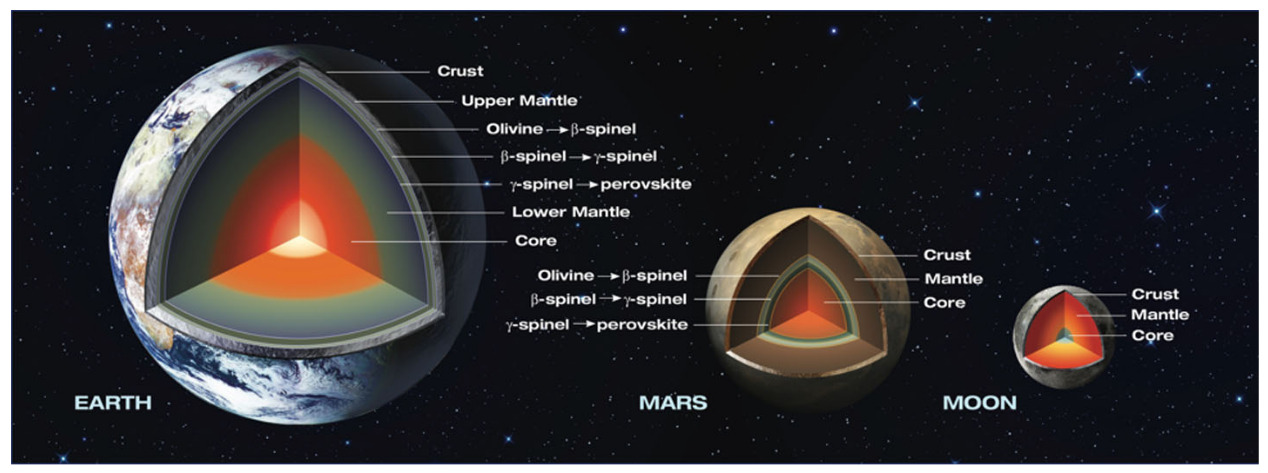
\includegraphics[width=10cm]{images/mars/smls19a}
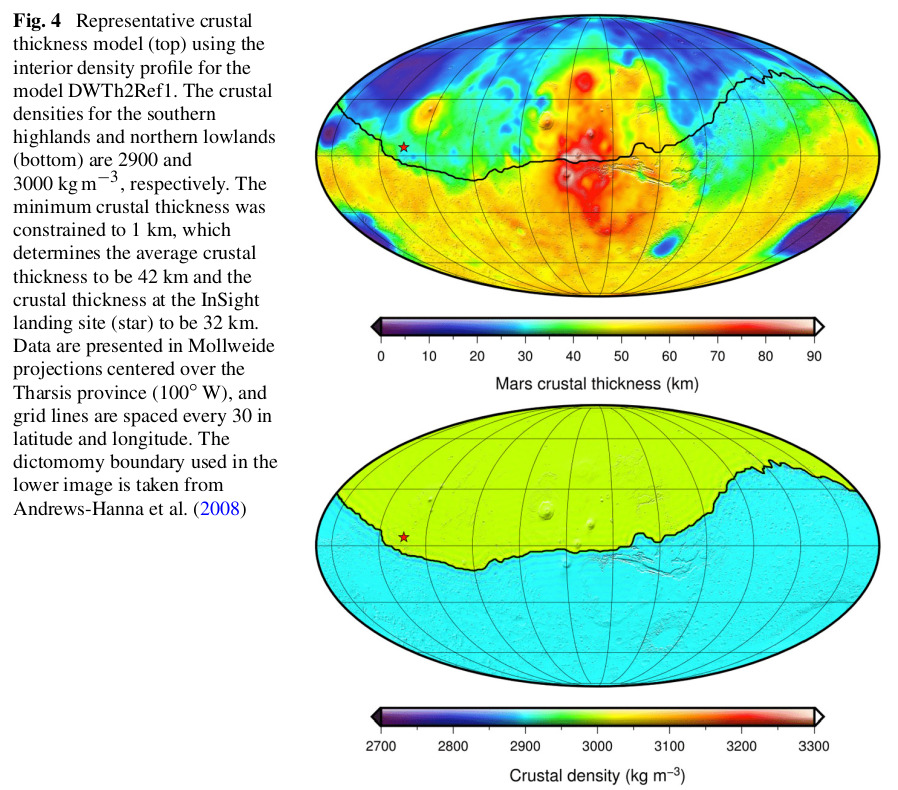
\includegraphics[width=6cm]{images/mars/smls19b}
\end{center}

%------------------------------
\item \fullcite{knpb21}

\begin{displayquote}
{\color{darkgray}
we determine the structure of the
crust beneath the InSight landing site on Mars using both marsquake recordings and the ambient wavefield.
By analyzing seismic phases that are reflected and converted at subsurface interfaces, we find that the
observations are consistent with models with at least two and possibly three interfaces. If the second interface
is the boundary of the crust, the thickness is 20 $\pm$ 5 kilometers, whereas if the third interface 
is the boundary, the thickness is 39 $\pm$ 8 kilometers. 
Global maps of gravity and topography allow extrapolation of this point
measurement to the whole planet, showing that the average thickness of the martian crust lies between 24 and
72 kilometers. Independent bulk composition and geodynamic constraints show that the thicker model is
consistent with the abundances of crustal heat-producing elements observed for the shallow surface,
whereas the thinner model requires greater concentration at depth.
}
\end{displayquote}

\begin{center}
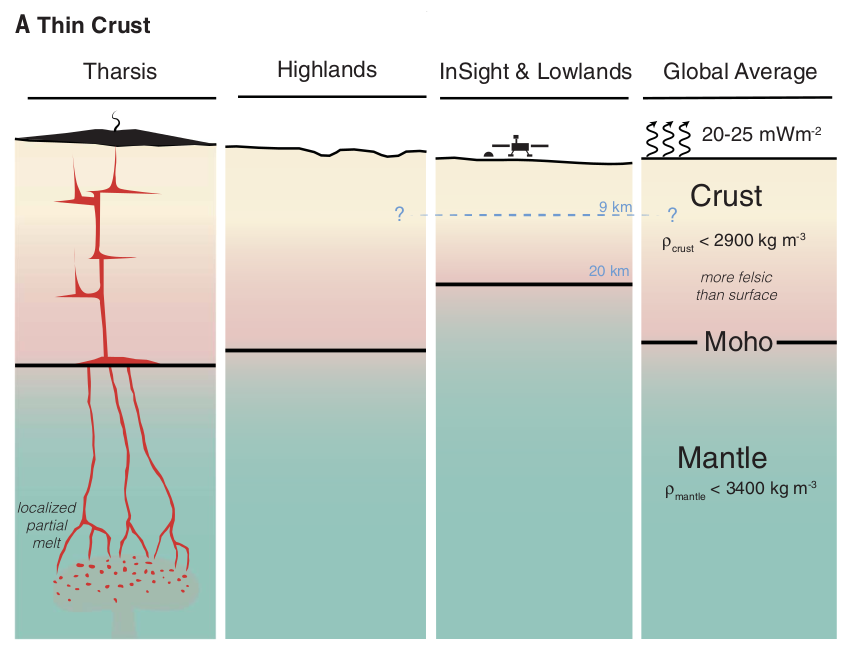
\includegraphics[width=8cm]{images/mars/knpb21a}
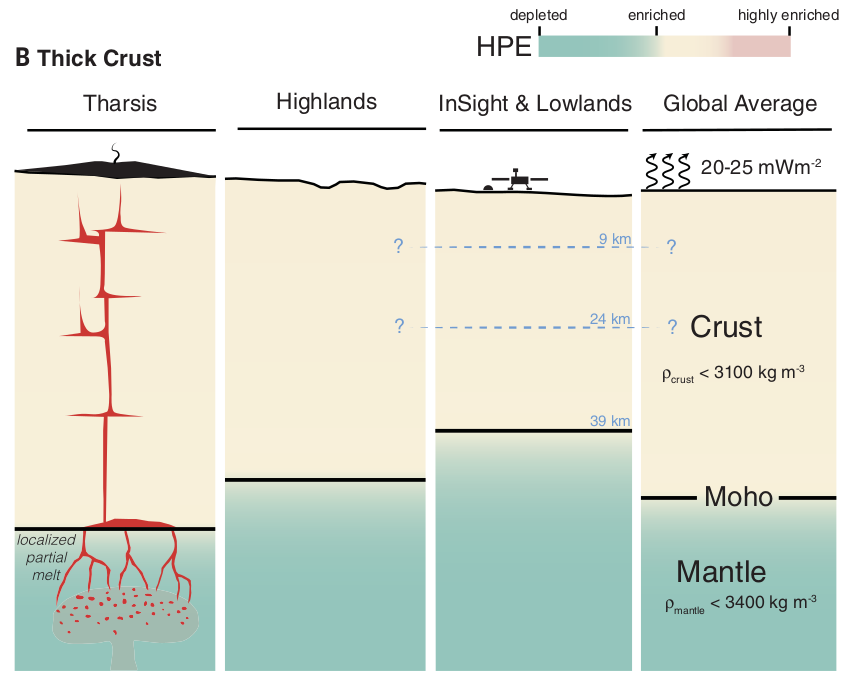
\includegraphics[width=8cm]{images/mars/knpb21b}
\end{center}

%------------------------------
\item \fullcite{stkb21}

\begin{displayquote}
{\color{darkgray}
We
detected reflections of seismic waves from the core-mantle boundary of Mars using InSight seismic data
and inverted these together with geodetic data to constrain the radius of the liquid metal core to 
1830 $\pm$ 40 kilometers. The large core implies a martian mantle mineralogically similar to the terrestrial upper
mantle and transition zone but differing from Earth by not having a bridgmanite-dominated lower
mantle. We inferred a mean core density of 5.7 to 6.3 grams per cubic centimeter, which requires a
substantial complement of light elements dissolved in the iron-nickel core.
}
\end{displayquote}

\begin{center}
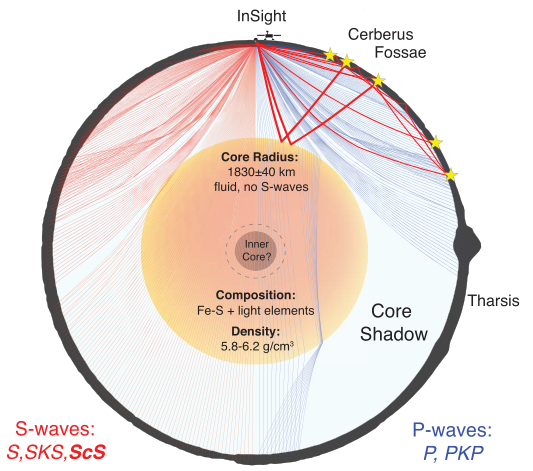
\includegraphics[width=7cm]{images/mars/stkb21}
\end{center}

\end{itemize}

